\documentclass[conference]{IEEEtran}
\usepackage{cite}
\usepackage{amsmath,amssymb,amsfonts}
\usepackage{algorithmic}
\usepackage{booktabs}
\usepackage{caption}
\usepackage{graphicx}
\usepackage{listings}
\usepackage{textcomp}
\usepackage{xcolor}
\def\BibTeX{{\rm B\kern-.05em{\sc i\kern-.025em b}\kern-.08em
    T\kern-.1667em\lower.7ex\hbox{E}\kern-.125emX}}
\begin{document}


\title{CENG435 Term Project, Part 2\\
}

\author{\IEEEauthorblockN{Doruk Coskun}
\IEEEauthorblockA{
}
\and
\IEEEauthorblockN{Yagmur Oymak}
\IEEEauthorblockA{
}
}

\maketitle

\section{Introduction}

In our CENG435 Term Project Part 2 we have implemented a reliable data transfer protocol on top of UDP in Application layer. To achieve this we have implemented checksum, SEQ counter and timer mechanisms. On top of that, to optimize data transfer rate we have added pipelining and multi-homing strategies. We have implemented Go-Back-N as our pipelining protocol and utilized both links to send data to Destination.

\section{Setting Up the Environment}
 Routing table implementation, config file max size, tc netem experimentation set up.

In the first part of the assignment we used applications on the routers to forward the packets. In the second part we have set the forwarding tables in the routers. This way Kernal handles the forwarding and we were able to got rid of the application layer forwarding. You can check the detailed explanation of how we set the forwarding tables in the README.md file.

We use config files to determine the size of the packets. It can be adjusted through those files. It is important to keep in mind that our packet headers are 20 bytes and the minimum packet size must be larger than that.

We have written our own shell scripts which send the codes to the nodes and set the netem/tc corruption, loss, reorder and delay parameters in the nodes.

Then we can run our codes and start the experiments.

\section{Design Decisions}

In our design, we have decided to implement Go-Back-N protocol and added header to our packets. The size of our headers are 20 bytes in total. The first 4 bytes indicate the SEQ number of the packets and the remaining 16 bytes are used for MD5 Checksum. We have decided that including the packet length to the header was redundant since our Broker and Destination send and read the packets by a predetermined maximum size which is declared in the config file. Packets size less than that do not cause any problems.

When the scripts are executed, 5MB file is sent to Broker from Source over TCP. Broker packages the bytes received from byte stream into packets and sends them to Destination over both routers using UDP. Routers forward the packets to Destination as we have defined in their forwarding tables. Destination expects the packets from both routers. When a packet is received, Destination checks its SEQ number and accepts the packet with the correct SEQ number. When a packet with the expected SEQ number is received, SEQ number counter in Destination is incremented. Regardless whether a packet is accepted or not, an ACK message is sent back to Broker, informing Broker the current SEQ number in the Destination. Broker adjusts its Window according to the SEQ number of the received ACK and sends new packets.

Broker also has a timer. When the timer expires before Broker receives an ACK, it sends the packets in the Window again. Timer is resetted and Window is moved if a packet with SEQ number higher than the Base SEQ in Broker is received.

Destination is a synchronized multithreaded application. Sockets which are binded to two different interfaces are run on these threads and awaits packets from different routers. When a packet with expected SEQ number is received, it is written to a file. SEQ number variable is secured with threading lock, preventing concurrent access to the variable by different threads. When a packet is received, regardless of its contents, appropriate ACK packet is sent back, informing Broker about the current SEQ number in the Destination.

Timer in Broker handles the cases where the packets are lost. Our MD5 Checksum mechanism protects against corrupted packets and our SEQ number implementation preserves the integrity of the file when packets are received out of order.

\subsection{Detailed Explanation of Broker Implementation}

TODO

\section{Experiments}

In our experiments we have plotted loss, corruption and reordering tests. We have changed netem/tc properties of the links between Broker and Destination while conducting these tests. For each property we have plotted 3 different scenarios. 

\subsection{Packet Loss Test}\label{AA}

For the packet loss tests we have set the loss and delay properties of the links. 3 different scenarios we have plotted can be seen here:

\begin{itemize}
    \item \textbf{Configuration 1:} 3ms delay and $\%0.5$ loss
    \item \textbf{Configuration 2:} 3ms delay and $\%10$ loss
    \item \textbf{Configuration 3:} 3ms delay and $\%20$ loss
\end{itemize}

\subsection{Packet Corruption Test}\label{AA}

For the packet corruption tests we have set the corrupt and delay properties of the links. 3 different scenarios we have plotted can be seen here:

\begin{itemize}
    \item \textbf{Configuration 1:} 3ms delay and $\%0.2$ corrupt
    \item \textbf{Configuration 2:} 3ms delay and $\%10$ corrupt
    \item \textbf{Configuration 3:} 3ms delay and $\%20$ corrupt
\end{itemize}

\subsection{Packet Reordering Test}\label{AA}

For the packet reordering tests we have set the reorder and delay properties of the links. 3 different scenarios we have plotted can be seen here:

\begin{itemize}
    \item \textbf{Configuration 1:} 3ms delay and $\%1$ reorder
    \item \textbf{Configuration 2:} 3ms delay and $\%10$ reorder
    \item \textbf{Configuration 3:} 3ms delay and $\%35$ reorder
\end{itemize}

\subsection{Emulated Network Delay Test}\label{AA}

In our experiments we have plotted the 3 scenarios given in the homework text:

 You will change the loss, corruption and reordering property of the links explained below. 

\begin{itemize}
    \item \textbf{Experiment 1:} 1ms $\pm$ 5ms
    \item \textbf{Experiment 2:} 20ms $\pm$ 5ms
    \item \textbf{Experiment 3:} 60ms $\pm$ 5ms
\end{itemize}
You can find end-to-end delay results of these experiments in Figure~\ref{fig:graph}.

Apart from these experiments we have also observed the end-to-end delay without any network delay emulations. In the first glance we could not make much sense of the results. That's why we have concluded to  make even more test with different emulated network delays and compare those results. Remaining experiments, their mean delays, jitter delays and the estimated end-to-end delay can be seen below:

\begin{itemize}
    \item \textbf{Experiment 0:} 0 emulated delay, end-to-end delay: 20ms
    \item \textbf{Experiment 4:} 1ms $\pm$ 1 ms, end-to-end delay: 20ms
    \item \textbf{Experiment 5:} 5ms $\pm$ 1ms, end-to-end delay: 20ms
    \item \textbf{Experiment 6:} 7.5ms $\pm$ 1ms, end-to-end delay: 20ms
    \item \textbf{Experiment 7:} 10ms $\pm$ 1ms, end-to-end delay: 20ms
    \item \textbf{Experiment 8:} 12.5ms $\pm$ 1ms, end-to-end delay: 25ms
    \item \textbf{Experiment 9:} 15ms $\pm$ 1ms, end-to-end delay: 30ms
    \item \textbf{Experiment 10:} 20ms $\pm$ 1ms, end-to-end delay: 40ms
    \item \textbf{Experiment 11:} 50ms $\pm$ 1ms, end-to-end delay: 100ms
    \item \textbf{Experiment 12:} 100ms $\pm$ 1ms, end-to-end delay: 200ms
\end{itemize}

For our experiments we have first set the network emulation delays. We have collected the end-to-end delay data of 1100 packets for each experiment. Using these data we have calculated the mean delays and 95\% confidence intervals.

Figure~\ref{fig:graph} illustrates our experimental results for Experiments 0, 1, 2 and 3.
We calculated the 95\% confidence intervals as 19.2 to 19.6 for Experiment 0,
19.1 to 19.7 for Experiment 1, 40.6 to 41.2 for Experiment 2 and 120.9 to 121.1
for Experiment 3. Table~\ref{table:data} shows the summary of these results.

In the light of all the experiments, we have concluded that when the netem/tc delay is set lower than the actual end-to-end delay, it does not effect the end-to-end delay of the packets. We observed looking at the Experiments 1, 4, 5, 6, and 7 that end-to-end delay remains the same even though netem/tc delay was increased gradually but did not exceed the actual end-to-end delay. When, the netem/tc delay is bigger than the actual end-to-end delay, netem/tc delay is not added on the top of the actual delay but it extends the delay at the each node to the set amount as it can be seen in the Experiments 8, 9, 10, 11 and 12. Since the delay between Source and Broker is negligible (Link capacity is 100 times of the other links in the network) netem/tc delay set on the UDP nodes, determine the total end-to-end delay.

\begin{figure}
    \centering
    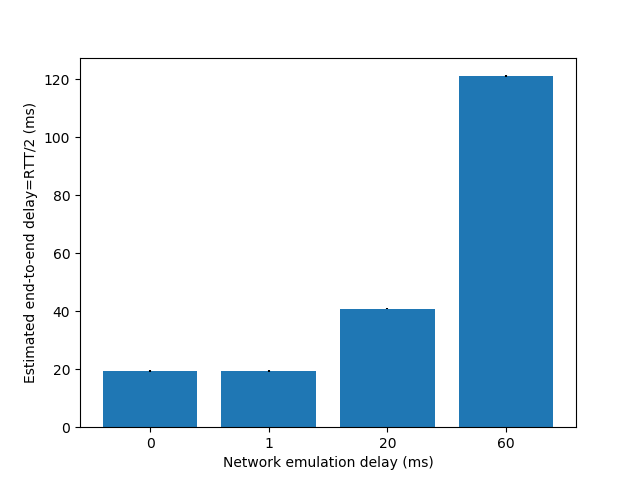
\includegraphics[scale=0.6]{graphics/plt}
    \caption{Network emulation delay vs.\ end-to-end delay}\label{fig:graph}
\end{figure}

Having read the manual of netem/tc we had hard time making sense about the results we got from the experiments. We were expecting to see our end-to-end delay to increase by network emulation delay for each network delay emulated node. Namely for each pass through broker and router. As an example when we set netem/tc delay to 20ms with 5ms jitter we expected to see the delay: $20ms$ (actual delay) $+$ $20ms$ (delay from broker) $+$ $20ms$ (delay from router 1) $=$ $60ms$.

Moreover, with or without emulated delays, the first few packets sent would return
very quickly (in the order of a few milliseconds) but as the source sent more packets,
the delay would quickly increase to a higher value (around 39 milliseconds round trip time with no
emulated delay). To make sense of this, we ran some experiments using \textbf{ping}
with different packet sizes and time intervals. Curiously, a similar pattern was observed
with certain configurations; first few packets would arrive in a few milliseconds, then
after a point, packets would be delayed and started to drop. This may be interpreted
as the link capacity being exceeded; however this should not have happened in our test programs
because the source does not send any new packets until the feedback of the last packet it had sent
returned. The source should not be able to congest the link, yet it does
(or an implementation error we could not detect causes this strange pattern).

\begin{table}
    \centering
    \begin{tabular}{c c c c}
        \toprule
        NetEm delay & $\mu$ & $\sigma$ & Error \\
        $0ms$   &    $19.4ms$   &   $3.43ms$    &   $0.203ms$ \\
        $1ms$   &    $19.4ms$   &   $4.47ms$    &   $0.264ms$ \\
        $20ms$   &    $40.9ms$   &   $4.92ms$    &   $0.291ms$ \\
        $60ms$   &    $121ms$   &   $4.99ms$    &   $0.295ms$ \\
        \bottomrule
    \end{tabular}\label{table:data} \\
    \caption{Summary of experimental data}\label{table:data}
\end{table}

\end{document}
